\documentclass[border=10pt]{standalone}
\usepackage{pgfplots}
\pgfplotsset{compat=1.17}
\begin{document}
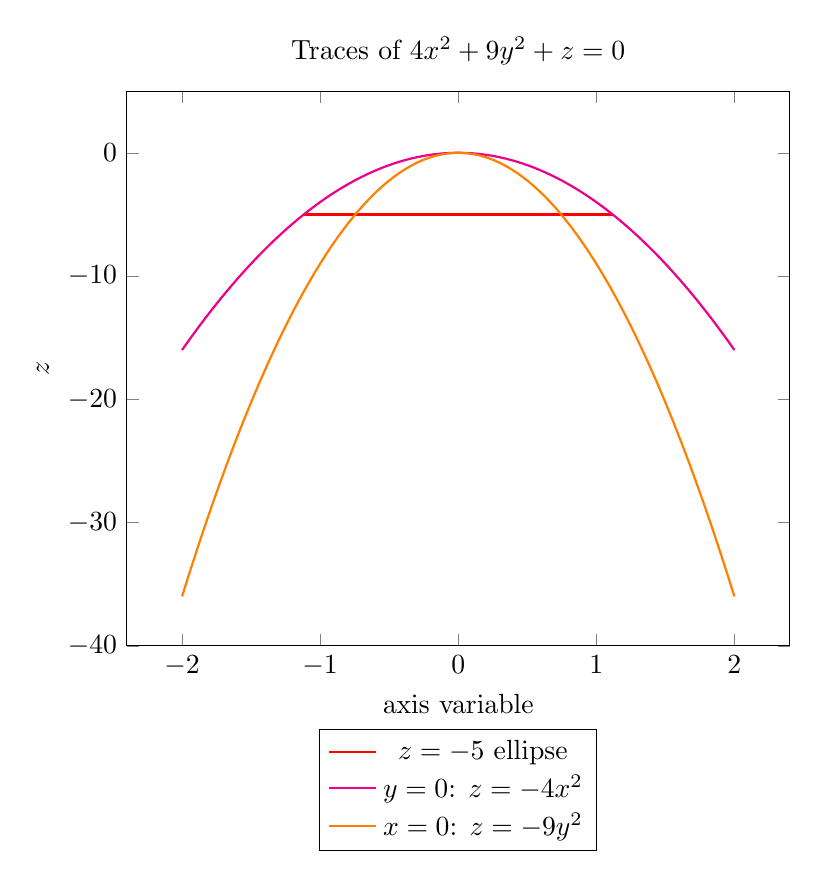
\begin{tikzpicture}
\begin{axis}[
    width=10cm,
    xlabel={axis variable}, ylabel=$z$,
    ymin=-40, ymax=5,
    legend style={at={(0.5,-0.15)}, anchor=north, legend columns=1},
    title={Traces of $4x^2+9y^2+z=0$},
    domain=-2:2,
    samples=100,
]
\addplot[red, thick, domain=0:360, variable=\t]
    ({sqrt(5)/2*cos(\t)}, -5);
\addlegendentry{$z=-5$ ellipse}
\addplot[magenta, thick] { -4*x^2 };
\addlegendentry{$y=0$: $z=-4x^2$}
\addplot[orange, thick] { -9*x^2 };
\addlegendentry{$x=0$: $z=-9y^2$}
\end{axis}
\end{tikzpicture}
\end{document}
